% Template:     Informe LaTeX
% Documento:    Archivo de ejemplo
% Versión:      7.0.0 (23/06/2020)
% Codificación: UTF-8
%
% Autor: Pablo Pizarro R.
%        Facultad de Ciencias Físicas y Matemáticas
%        Universidad de Chile
%        pablo@ppizarror.com
%
% Manual template: [https://latex.ppizarror.com/informe]
% Licencia MIT:    [https://opensource.org/licenses/MIT]

% ------------------------------------------------------------------------------
% NUEVA SECCIÓN
% ------------------------------------------------------------------------------
% Las secciones se inician con \section, si se quiere una sección sin número se
% pueden usar las funciones \sectionanum (sección sin número) o la función
% \sectionanumnoi para crear el mismo título sin numerar y sin aparecer en el índice

\newcommand{\explorelite}{\textit{explore\_lite}}
\newcommand{\movebase}{\textit{move\_base}}

\section{Pregunta 1}

\subsection{Parte a.-}

Se construyó el bloque de transformada $abc$ a $dq$ de manera análoga para las señales de voltaje y corriente. Externamente el bloque se ve así:

\begin{figure}
    \centering
    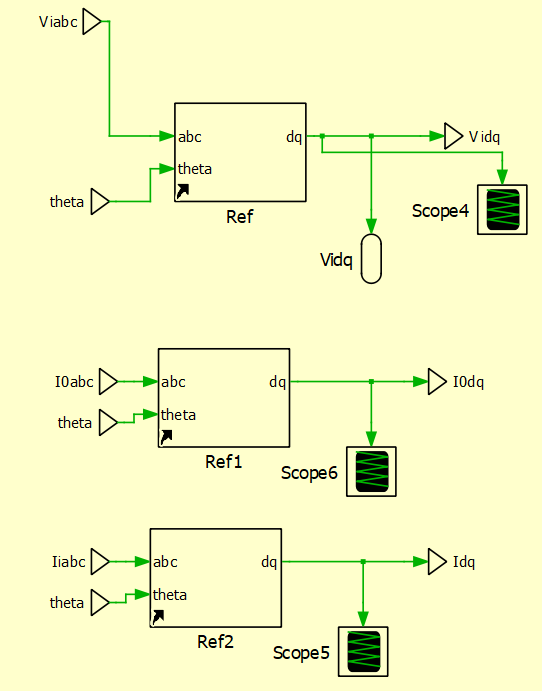
\includegraphics[width=0.5\linewidth]{Tarea 1/report/imagenes/p1a/transformadaporfuera.png}
    \caption{Perspectiva externa del bloque de la transformada $abc$-$dq$.}
    \label{transformadaporfuera}
\end{figure}

Dentro del bloque, se puede visualizar lo siguiente:

\begin{figure}
    \centering
    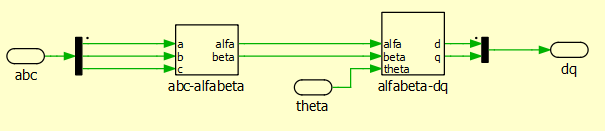
\includegraphics[width=0.5\linewidth]{Tarea 1/report/imagenes/p1a/transformadapordentro.png}
    \caption{Perspectiva interna del bloque de la transformada $abc$-$dq$.}
    \label{transformadapordentro}
\end{figure}

A partir de la Figura \ref{transformadapordentro}, se pueden ver los bloques de transformada $abc$-$\alpha\beta$ y $\alpha\beta$-$dq$. Estos bloques se armaron de la siguiente forma:

\begin{itemize}
    \item $abc$-$\alpha\beta$:

    \begin{figure}
       \centering
       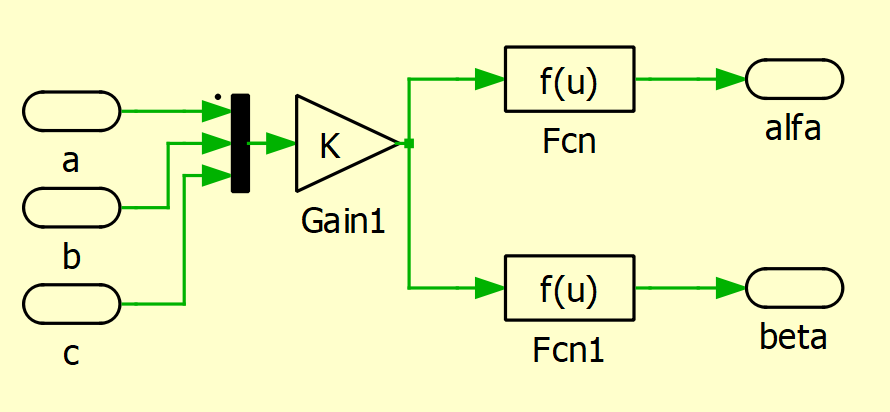
\includegraphics[width=0.5\linewidth]{Tarea 1/report/imagenes/p1a/abc-alphabetha.png}
       \caption{Bloque de transformada $abc$-$\alpha\beta$.}
       \label{abc-alphabetha}
    \end{figure}

    \begin{figure}
       \centering
       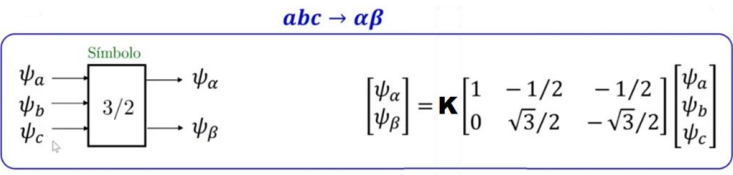
\includegraphics[width=0.5\linewidth]{Tarea 1/report/imagenes/p1a/formulaabc-alphabetha.png}
       \caption{Transformación matemática $abc$-$\alpha\beta$.}
       \label{formulaabc-alphabetha}
    \end{figure}

    De acuerdo a lo visto en clases, a las señales $abc$ se les aplicó la transformación que se visualiza en la Figura \ref{formulaabc-alphabetha} para dar origen al dominio $\alpha\beta$ como se puede ver en la Figura \ref{abc-alphabetha}, donde el valor de $K$ fue inicializado en $\frac{2}{3}$, el bloque ``Fcn'' equivale a las operaciones matemáticas que dan origen a la primera fila de la matriz $\alpha\beta$ y el bloque ``Fcn1''  equivale a las operaciones matemáticas que dan origen a la segunda fila de la matriz $\alpha\beta$.

    \item $\alpha\beta$-$dq$:

    \begin{figure}
       \centering
       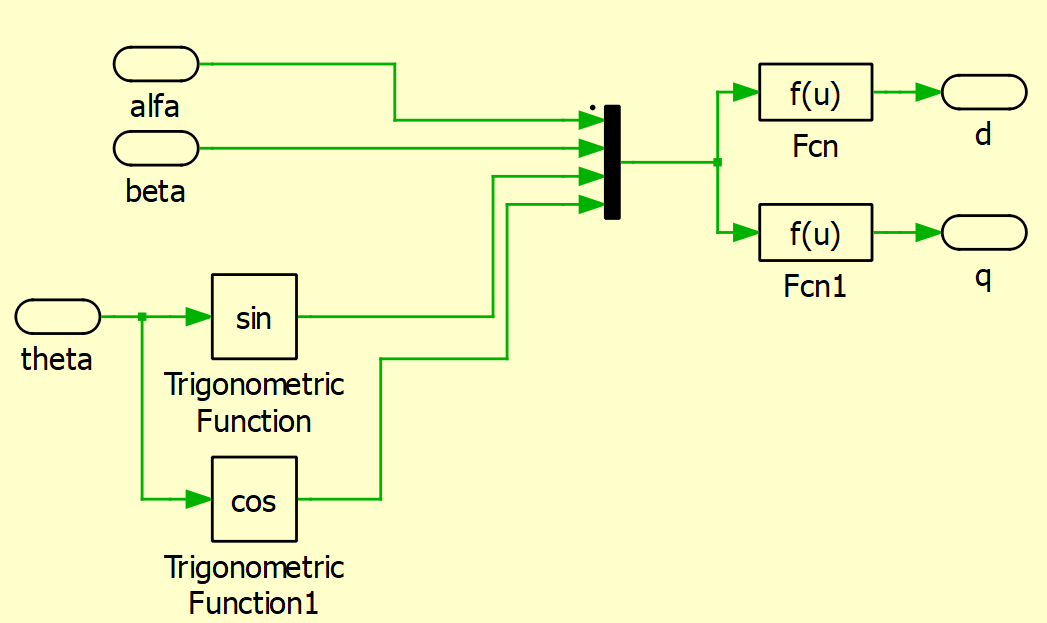
\includegraphics[width=0.5\linewidth]{Tarea 1/report/imagenes/p1a/alphabetha-dq.png}
       \caption{Bloque de transformada $\alpha\beta$-$dq$.}
       \label{alphabetha-dq}
    \end{figure}

    \begin{figure}
       \centering
       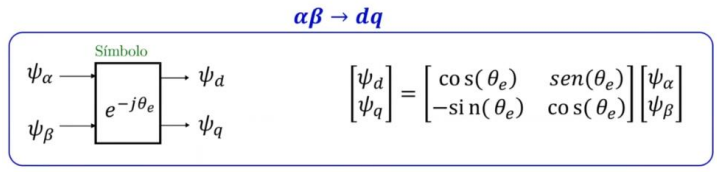
\includegraphics[width=0.5\linewidth]{Tarea 1/report/imagenes/p1a/formulaalphabetha-dq.png}
       \caption{Transformación matemática $\alpha\beta$-$dq$.}
       \label{formulaalphabetha-dq}
    \end{figure}

    De acuerdo a lo visto en clases, a las señales $\alpha\beta$ se les aplicó la transformación que se visualiza en la Figura \ref{formulaalphabetha-dq} para dar origen al dominio $dq$ como se puede ver en la Figura \ref{alphabetha-dq}, donde el bloque ``Fcn'' equivale a las operaciones matemáticas que dan origen a la primera fila de la matriz $dq$ y el bloque ``Fcn1''  equivale a las operaciones matemáticas que dan origen a la segunda fila de la matriz $dq$.
\end{itemize}

Cabe destacar que la idea de realizar la transformación del dominio $abc$ al dominio $dq$ es meramente por simplificación dado que se permite tratar los valores de voltaje y corriente como variables de corriente continua (DC).

\subsection{Parte b.-}

Utilizando las coordenadas $dq$, se creó el siguiente bloque capaz de hacer el cálculo de potencia activa y reactiva:

\begin{figure}
    \centering
    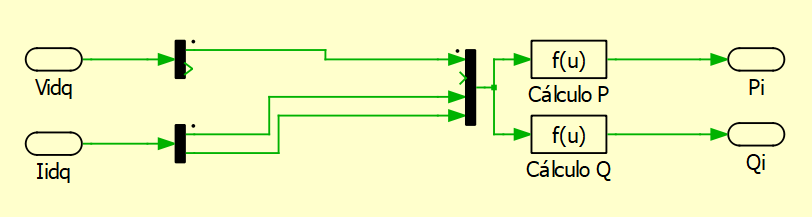
\includegraphics[width=0.5\linewidth]{Tarea 1/report/imagenes/p1b/bloquepq.png}
    \caption{Bloque que calcula la potencia activa y reactiva en base a las variables de voltaje corriente en el dominio $dq$.}
    \label{bloquepq}
\end{figure}

Como se puede visualizar en la Figura \ref{bloquepq}, el multiplexor tiene 4 entradas pero la segunda no recibe nada, esto ocurre debido a que el al alinear el sistema de coordenadas $dq$ con la dirección de la tensión (en particular, con el eje $d$), se logra que el voltaje en el eje $q$ sea 0, lo cual permite una separación clara entre la potencia activa y la reactiva, simplificando el control de la potencia en sistemas de conversión de energía. En otras palabras, se requiere que el voltaje en el eje $q$ sea 0. Luego, se siguen las siguientes fórmulas para el cálculo de P y Q:

\begin{equation}
    P = kv_{d}i_{d}
\end{equation}

\begin{equation}
    Q = -kv_{d}i_{q}
\end{equation}

Estas fórmulas se encuentran contenidas en los bloques ``Cálculo P'' y ``Cálculo Q'' respectivamente.

\subsection{Parte c.-}

Externamente, el bloque dentro del diagrama se puede visualizar de la siguiente forma:

\begin{figure}
   \centering
   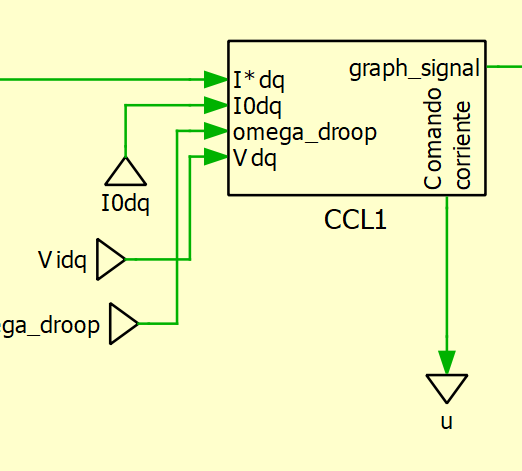
\includegraphics[width=0.5\linewidth]{Tarea 1/report/imagenes/p1c/ccl bloque externo.png}
   \caption{Perspectiva externa del bloque de control del lazo de corriente.}
   \label{ccl externo}
\end{figure}

Internamente, se utilizó un control con términos cruzados visto en cátedra, tal como se puede ver en la siguiente figura:

\begin{figure}
   \centering
   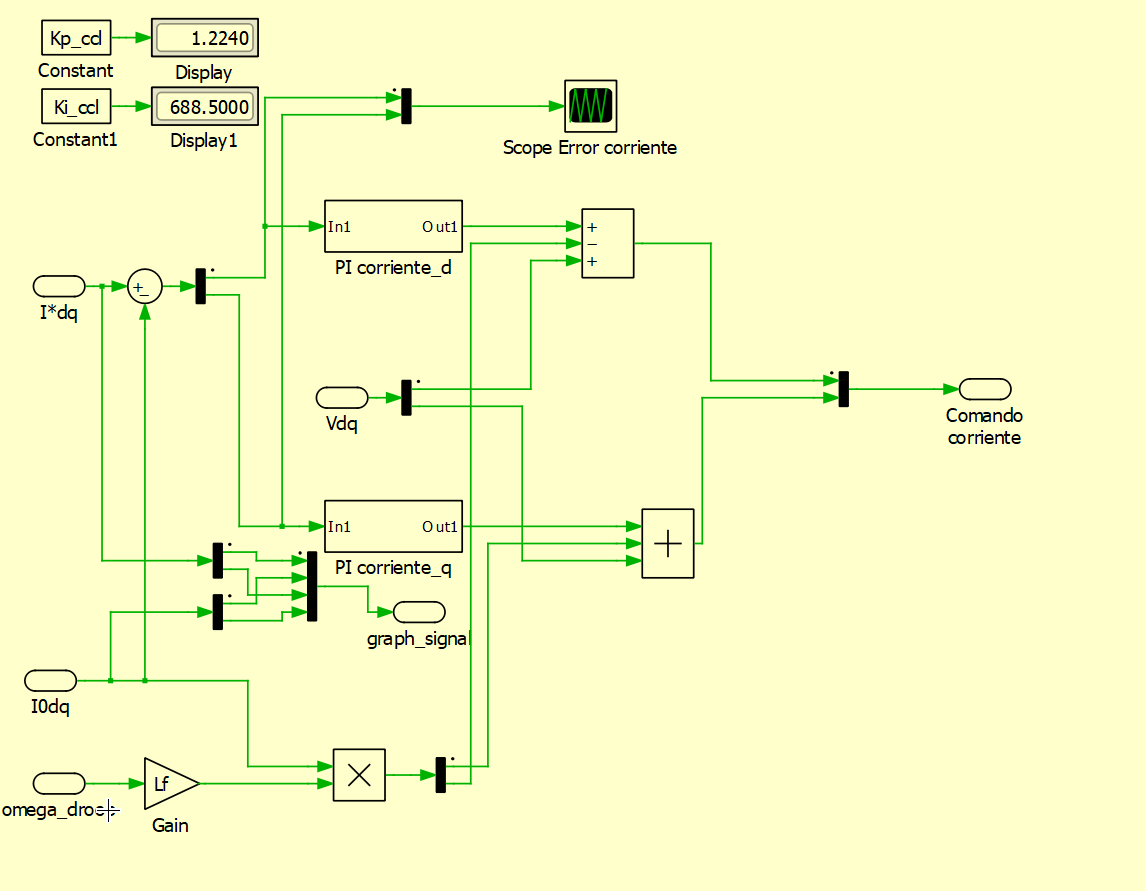
\includegraphics[width=0.5\linewidth]{Tarea 1/report/imagenes/p1c/ccl bloque interno.png}
   \caption{Perspectiva interna del bloque de control del lazo de corriente.}
   \label{ccl interno}
\end{figure}

De acuerdo a lo visto en clases, al modelo físico se le dio de entrada un escalón con el fin de observar su comportamiento, de esta manera fue posible estipular los valores de las constantes proporcionales e integrales de los controladores PI para cada entrada de corriente en el dominio $dq$, las fórmulas utilizadas para definir estos valores fueron:

\begin{equation}
    k_p^i = 2L\zeta w_{n}
\end{equation}

\begin{equation}
    k_i^i = Lw_{n}^2
\end{equation}

Utilizando estas fórmulas, se determinó que los valores de $k_p^i$ y $k_i^i$ son X y Z respectivamente, utilizando un $\zeta$ de U y un $w_{n}$ de O.

\subsection{Parte d.-}

Externamente, el bloque dentro del diagrama se puede visualizar de la siguiente forma:

\begin{figure}
   \centering
   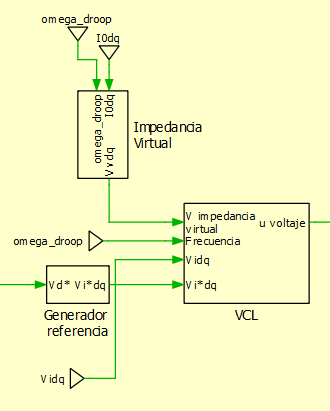
\includegraphics[width=0.5\linewidth]{Tarea 1/report/imagenes/p1d/vcl bloque externo.png}
   \caption{Perspectiva externa del bloque de control del lazo de voltaje.}
   \label{vcl externo}
\end{figure}

Internamente, se utilizó un control con términos cruzados visto en cátedra, tal como se puede ver en la siguiente figura:

\begin{figure}
   \centering
   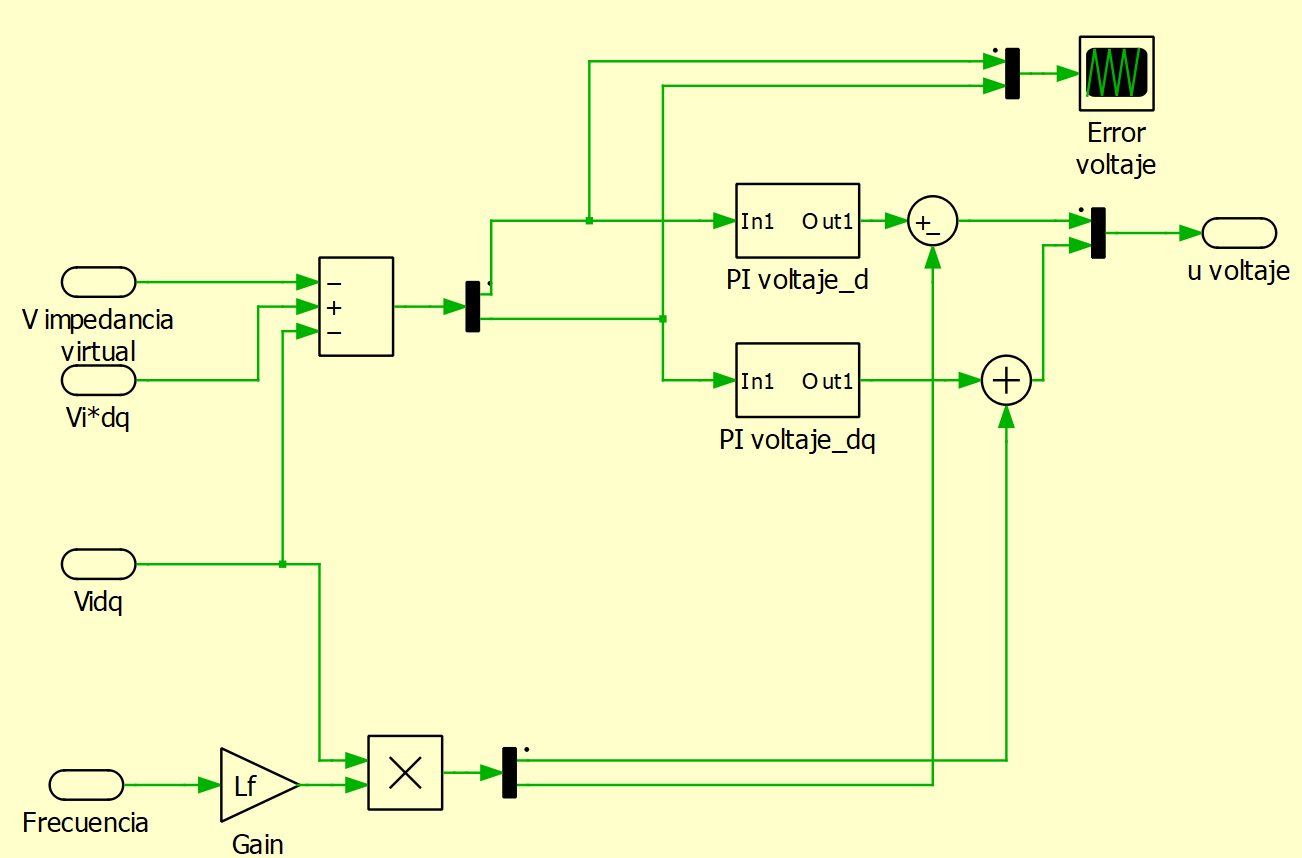
\includegraphics[width=0.5\linewidth]{Tarea 1/report/imagenes/p1d/vcl bloque interno.png}
   \caption{Perspectiva interna del bloque de control del lazo de voltaje.}
   \label{vcl interno}
\end{figure}

De acuerdo a lo visto en clases, al modelo físico se le dio de entrada un escalón con el fin de observar su comportamiento, de esta manera fue posible estipular los valores de las constantes proporcionales e integrales de los controladores PI para cada entrada de voltaje en el dominio $dq$, las fórmulas utilizadas para definir estos valores fueron:

\begin{equation}
    k_p^v = 2C\zeta w_{n}
\end{equation}

\begin{equation}
    k_i^v = Cw_{n}^2
\end{equation}

Utilizando estas fórmulas, se determinó que los valores de $k_p^v$ y $k_i^v$ son X y Z respectivamente, utilizando un $\zeta$ de U y un $w_{n}$ de O.

\subsection{Parte e.-}



\section{Pregunta 2}

\subsection{Parte a.-}

De acuerdo a lo visto en clases, para calcular la pendiente droop para cada potencia se debe seguir las siguientes fórmulas:

\begin{equation}
    M_p = \frac{\Delta w}{P_{máx}}
\end{equation}

\begin{equation}
    M_q = \frac{\Delta w}{Q_{máx}}
\end{equation}

Por otro lado, al estar tratando la pendiente como un valor porcentual, se debe multiplicar por la frecuencia nominal y dividir por 100 a ambas pendientes para dejarlos como porcentajes de los valores nominales. A partir de esto, se obtuvo que las pendientes droop para P y Q toman los valores de -0.000166666667 y -0.00073333333 respectivamente.\\

Al realizar una simulación teniendo las 3 máquinas generadoras con la misma pendiente droop de potencia activa y reactiva, se obtuvieron los siguientes resultados:



De acuerdo a la simulación, la potencia...

\subsection{Parte b.-}

Siguiendo las instrucciones, se cambiaron las pendientes droop de potencia activa y reactiva de modo que cada unidad generadora tiene valores de pendientes distintas. De este modo, se obtuvieron los siguientes resultados:



De acuerdo a estas simulaciones, la potencia...

\subsection{Parte c.-}

Investigando lo pedido, en el artículo 5-62 de la Norma Técnica de Seguridad y Calidad de Servicio (NTSyCS) estrenada en Septiembre del 2020, se estipula que:\\

La evaluación del desempeño del Control de Frecuencia del SI se efectuará a través del cálculo del factor FECF para cada hora k, el cual se define a través de la siguiente expresión:

\begin{equation}
    FECF(k) = 1 - \abs{\frac{\Delta f^*_{máx}(k)}{\Delta f_{máx}}}
\end{equation}

Donde:

\begin{itemize}
    \item $\Delta f^*_{máx}(k)$: Desviación máxima instantánea del valor filtrado de medición de la frecuencia.
    \item $\Delta f_{máx}$: Desviación máxima de frecuencia en estado permanente que agota la totalidad de la reserva asociada al Control Primario de Frecuencia y el Control Rápido de Frecuencia.
\end{itemize}

De acuerdo a esto, la pendiente máxima recomendada será la que entregue un FECF lo más cercana a 1 dado que este será el que entregará el mejor desempeño del Control de Frecuencia. Para lograr esto, lo que se requiere es que se tenga un $\Delta f^*_{máx}(k)$ lo más pequeño posible y un $\Delta f_{máx}$ lo más grande posible.

\section{Pregunta 3}

\subsection{Parte a.-}

Se diseñó un PLL de acuerdo a las especificaciones recomendadas en las clases del curso, este fue colocado en la red con el fin de medir su frecuencia, el diseño se encuentra a continuación:

\begin{figure}
   \centering
   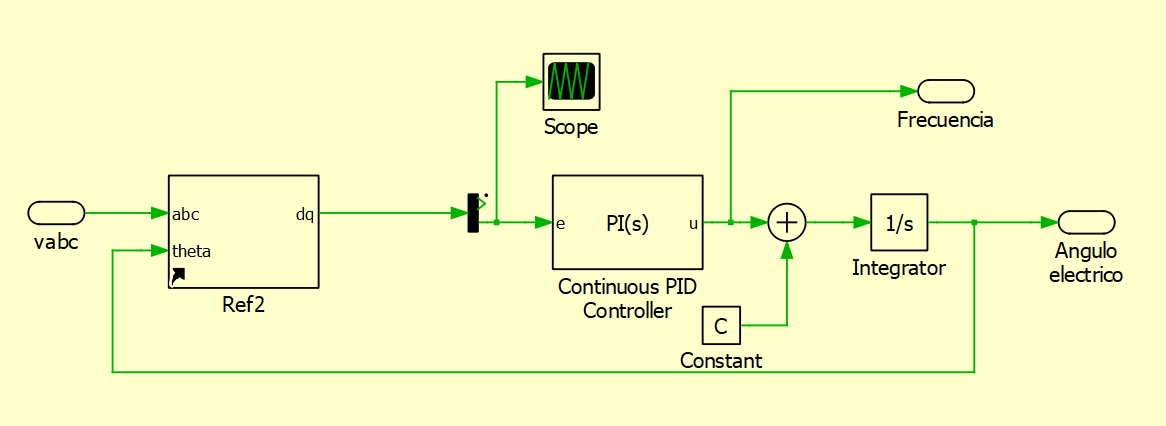
\includegraphics[width=0.5\linewidth]{Tarea 1/report/imagenes/p3a/pllred.png}
   \caption{Diseño PLL.}
   \label{diseñopll}
\end{figure}

El controlador PI utilizó las fórmulas:

\begin{equation}
    k_p^v = 2\zeta w_{n}
\end{equation}

\begin{equation}
    k_i^v = w_{n}^2
\end{equation}

Donde los valores utilizados para el coeficiente de amortiguamiento $\zeta$ y la frecuencia natural $w_{n}$ fueron 0.82 y 25 Hz respectivamente.\\

En base a esto, se realizó una simulación donde las 3 unidades de generación parten desconectadas y luego se conectan las 3 al mismo tiempo, los resultados fueron los siguientes:



Las mediciones otorgadas por el PLL indican que la frecuencia de la red toma un valor entre los rangos de X y Z, esto implica que...

\subsection{Parte b.-}



\subsection{Parte c.-}



\subsection{Parte d.-}



\section{Extras}

\subsection{Parte a.-}



\subsection{Parte b.-}



